\documentclass[12pt,a4paper,oneside]{article}

\usepackage[utf8]{inputenc}
\usepackage[portuguese]{babel}
\usepackage[T1]{fontenc}
\usepackage{amsmath}
\usepackage{amsfonts}
\usepackage{amssymb}
\usepackage{graphicx}

\usepackage{xcolor}
% Definindo novas cores
\definecolor{verde}{rgb}{0.25,0.5,0.35}
\definecolor{jpurple}{rgb}{0.5,0,0.35}
% Configurando layout para mostrar codigos Java
\usepackage{listings}
\definecolor{mygreen}{rgb}{0,0.6,0}
\definecolor{mygray}{rgb}{0.5,0.5,0.5}
\definecolor{mymauve}{rgb}{0.58,0,0.82}

\lstdefinelanguage{JavaScript}{
  keywords={typeof, new, true, false, catch, function, return, null, catch, switch, var, if, in, while, do, else, case, break},
  keywordstyle=\color{blue}\bfseries,
  ndkeywords={class, export, boolean, throw, implements, import, this},
  ndkeywordstyle=\color{darkgray}\bfseries,
  identifierstyle=\color{black},
  sensitive=false,
  comment=[l]{//},
  morecomment=[s]{/*}{*/},
  commentstyle=\color{purple}\ttfamily,
  stringstyle=\color{red}\ttfamily,
  morestring=[b]',
  morestring=[b]",
}

\lstset{ %
  backgroundcolor=\color{white},   % choose the background color; you must add \usepackage{color} or \usepackage{xcolor}
  basicstyle=\small,        % the size of the fonts that are used for the code
  breakatwhitespace=false,         % sets if automatic breaks should only happen at whitespace
  breaklines=true,                 % sets automatic line breaking
  captionpos=b,                    % sets the caption-position to bottom
  commentstyle=\color{mygreen},    % comment style
  deletekeywords={...},            % if you want to delete keywords from the given language
  escapeinside={\%*}{*)},          % if you want to add LaTeX within your code
  extendedchars=true,              % lets you use non-ASCII characters; for 8-bits encodings only, does not work with UTF-8
  frame=single,	                   % adds a frame around the code
  keepspaces=true,                 % keeps spaces in text, useful for keeping indentation of code (possibly needs columns=flexible)
  keywordstyle=\color{blue},       % keyword style
  language=HTML,                 % the language of the code
  otherkeywords={*,...},           % if you want to add more keywords to the set
  numbers=left,                    % where to put the line-numbers; possible values are (none, left, right)
  numbersep=5pt,                   % how far the line-numbers are from the code
  numberstyle=\tiny\color{mygray}, % the style that is used for the line-numbers
  rulecolor=\color{black},         % if not set, the frame-color may be changed on line-breaks within not-black text (e.g. comments (green here))
  showspaces=false,                % show spaces everywhere adding particular underscores; it overrides 'showstringspaces'
  showstringspaces=false,          % underline spaces within strings only
  showtabs=false,                  % show tabs within strings adding particular underscores
  stepnumber=1,                    % the step between two line-numbers. If it's 1, each line will be numbered
  stringstyle=\color{mymauve},     % string literal style
  tabsize=2,	                   % sets default tabsize to 2 spaces
  title=\lstname,                   % show the filename of files included with \lstinputlisting; also try caption instead of title
  moredelim=**[is][\color{purple}]{@}{@},
}

\author{\\Universidade Federal de Goiás (UFG) - Regional Jataí\\Bacharelado em Ciência da Computação \\Física para Ciência da Computação \\Esdras Lins Bispo Jr.}

\title{\sc \huge Primeiro Teste}

\date{11 de outubro de 2016}

\begin{document}

\maketitle

{\bf ORIENTAÇÕES PARA A RESOLUÇÃO}

\footnotesize

\begin{itemize}
	\item A avaliação é individual, sem consulta;
	\item A pontuação máxima desta avaliação é 10,0 (dez) pontos, sendo uma das 05 (cinco) componentes que formarão a média final da disciplina: dois testes, duas provas e exercícios-bônus;
	\item A média final ($MF$) será calculada assim como se segue
	\begin{eqnarray}
		MF & = & MIN(10, S) \nonumber \\
		S & = & (\sum_{i=1}^{4} 0,2.T_i ) + 0,2.P  + EB \nonumber
	\end{eqnarray}
	em que 
	\begin{itemize}
		\item $S$ é o somatório da pontuação de todas as avaliações,
		\item $T_i$ é a pontuação obtida no teste $i$,
		\item $P$ é a pontuação obtida na prova, e
		\item $EB$ é a pontuação total dos exercícios-bônus.
	\end{itemize}
	\item O conteúdo exigido compreende os seguintes pontos apresentados no Plano de Ensino da disciplina: (1) Fundamentos Matemáticos e (2) Medidas Físicas e Vetores.
\end{itemize}


\begin{center}
	\fbox{\large Nome: \hspace{10cm}}
	\fbox{\large Assinatura: \hspace{9cm}}
\end{center}

\newpage

\normalsize

\begin{enumerate}

	\item (5,0 pt) {\bf (Halliday 1.15)} Três relógios digitais, A, B e C, funcionam com velocidades diferentes e não têm leituras simultâneas de zero. A Figura 1 mostra leituras simultâneas de pares dos relógios em quatro ocasiões. (Na primeira ocasião, por exemplo, B indica 25,0 s e C indica 92,0 s.) Se o intervalo entre dois eventos é 600 s de acordo com o relógio A, qual é o intervalo entre os eventos 
	
	\begin{center}
		\begin{figure}[htb]
			\centering		
			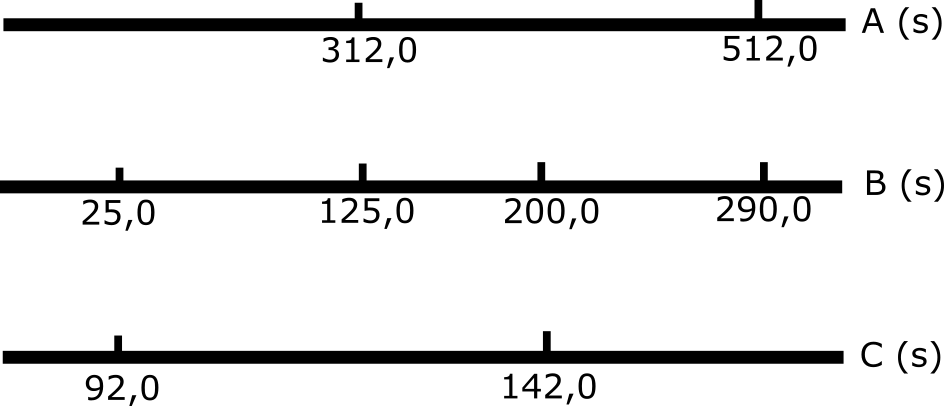
\includegraphics[scale=0.4]{images/hal13.png}
			\caption{Leitura simultânea de pares de relógios em quatro ocasiões (relógios A, B e C).}
		\end{figure}
	\end{center}
	
		\begin{enumerate}
			\item no relógio B, e
			
			\vspace{0.3cm}
			
			{\color{blue} Resposta:
			
				\begin{center}
					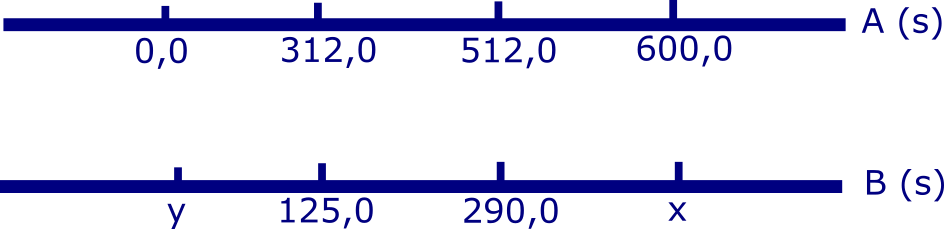
\includegraphics[scale=0.4]{images/resp-a.png}
				\end{center}
				\vspace{0.2cm}
				
				\begin{equation}
					\dfrac{600-0}{x-y} = \dfrac{512-312}{290-125}
				\end{equation}	
				
				O valor de $x-y$ (chamaremos de $\Delta_{xy}$) é o intervalo entre os eventos no relógio B. Logo, temos:							
				\begin{equation}
					\Delta_{xy} = \dfrac{600.(290-125)}{512-312} = 495 = 4,95 \times 10^2 \mbox{ s}
				\end{equation}
				
				
			}
			\item no relógio C?
			
			\vspace{0.3cm}
			
			{\color{blue} Resposta:
			
				\begin{center}
					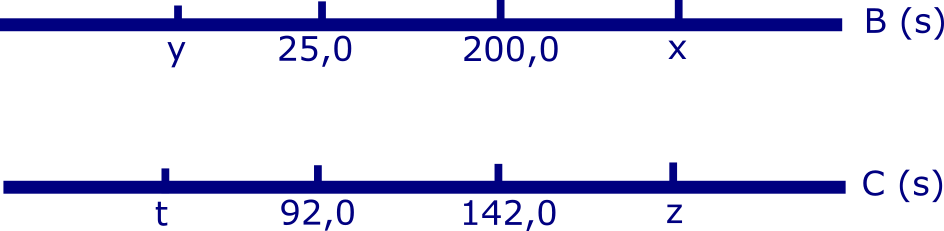
\includegraphics[scale=0.4]{images/resp-b.png}
				\end{center}
				\vspace{0.2cm}
				
				\begin{equation}
					\dfrac{x-y}{z-t} = \dfrac{200-25}{142-92}
				\end{equation}
				
				O valor de $x-y$ (chamaremos de $\Delta_{xy}$) é o intervalo entre os eventos no relógio B; e o valor de $z-t$ (chamaremos de $\Delta_{zt}$) é o intervalo entre os eventos no relógio C. Logo, temos:							
				\begin{equation}
					\Delta_{zt} = \dfrac{\Delta_{xy}.(142-92)}{200-25} = \dfrac{495.(142-92)}{200-25} \cong 141,43 \cong 1,41 \times 10^2 \mbox{ s} \nonumber
				\end{equation}
			}
		\end{enumerate}
	Verifique também se
		\begin{enumerate}
			\setcounter{enumii}{2}
			\item Quando o relógio A indica 400 s, qual é a indicação do relógio B?
			
			\vspace{0.3cm}
			
			{\color{blue} Resposta:
			
				\begin{center}
					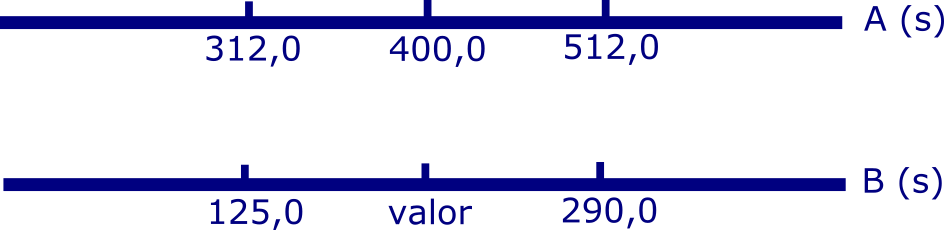
\includegraphics[scale=0.4]{images/resp-c.png}
				\end{center}
				\vspace{0.2cm}
				
				\begin{equation}
					\dfrac{512-312}{290-125} = \dfrac{400-312}{\mbox{valor} - 125}
				\end{equation}
				
				Ao isolarmos {\tt valor}, temos:							
				\begin{equation}
					\mbox{valor} = \dfrac{(400-312)(290-125)}{512-312} + 125 = 197,6 \cong 1,98 \times 10^2 \mbox{ s} \nonumber
				\end{equation}				
			}
			\item Quando o relógio C indica 15,0 s, qual é a indicação do relógio B?
			
			\vspace{0.3cm}
			
			{\color{blue} Resposta:
			
				\begin{center}
					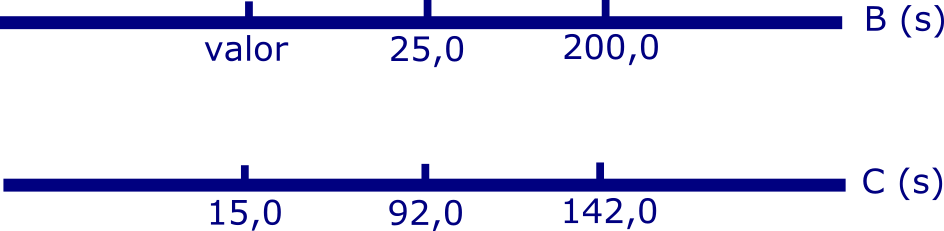
\includegraphics[scale=0.4]{images/resp-d.png}
				\end{center}
				\vspace{0.2cm}
				
				\begin{equation}
					\dfrac{200-\mbox{valor}}{142-15} = \dfrac{200-25}{142-92}
				\end{equation}
				
				Ao isolarmos {\tt valor}, temos:							
				\begin{equation}
					\mbox{valor} = 200 - \dfrac{(200-25)(142-15)}{142-92} = -244,5 \cong - 2,44 \times 10^2 \mbox{ s} \nonumber
				\end{equation}				
			}
		\end{enumerate}
	(Suponha que as leituras sejam negativas para instantes anteriores a zero.)
	
	\newpage
	
	\item (5,0 pt) Em JavaScript, crie um protótipo de objeto {\tt Particula} que tenha as propriedades (i) {\tt nome}, (ii) {\tt carga}, (iii) {\tt spin}, e (iv) {\tt descricao}. O {\tt nome} é uma cadeia; a {\tt carga} e o {\tt spin} são valores numéricos; e a {\tt descricao} é uma função que exibe, via {\tt console.log}, todas as demais propriedades de {\tt Particula}. Crie um objeto a partir de {\tt Particula}. Atribua valores para as propriedades ao seu gosto.
	
	\vspace{0.3cm}
	
	{\color{blue} Resposta: }

	\begin{lstlisting}[language=JavaScript]
function Particula(nome, carga, spin){
	this.nome = nome;
	this.carga = carga;
	this.spin = spin;
	this.descricao = function(){
		console.log("===DESCRICAO===");
		console.log("Nome: " + this.nome);
		console.log("Carga: " + this.carga);
		console.log("Spin: " + this.spin);
	};
}

particula1 = new Particula("atomo", 1, -1);
particula1.descricao();	//exibe os dados do objeto particula1
\end{lstlisting}
	
	\end{enumerate}
\end{document}